\documentclass[a4paper, 12pt]{article}
\usepackage{titling}
\usepackage{array}
\usepackage{booktabs}
\usepackage{enumitem}
\usepackage{graphicx}
\usepackage{hyperref}
\usepackage{amssymb}
\setlength{\heavyrulewidth}{1.5pt}
\setlength{\abovetopsep}{4pt}
\setlength{\parindent}{0pt}
\graphicspath{{.}}

\usepackage[margin=1in]{geometry}

% Must be after geometry
\usepackage{fancyhdr}
\pagestyle{fancy}
\fancyhf{}
\rhead{NN Homework 1}
\lhead{P.Lukin, I. Vishniakou, E. Ovchinnikova}
\cfoot{\thepage}

\setlength{\droptitle}{-5em}

\title{Neural Networks  \\
				- Homework 1 -}
\author{Petr Lukin, Ivan Vishniakou, Evgeniya Ovchinnikova}
\date{Lecture date: 26 September 2016}

\begin{document}

\maketitle

\section{Mind map}
Neural network (NN) is a parallel distributed system consisted of computing cells ("neurons") that is capable of storing and using experimental knowledge to model a brain in processes of certain tasks performance.

\begin{figure}[h]
  \centering
  \caption{S. Haykin, Neural Networks, chapter 1. Mind map (a zoomed version of the map is attached as NN.png file).\label{fig:mindMap}}
  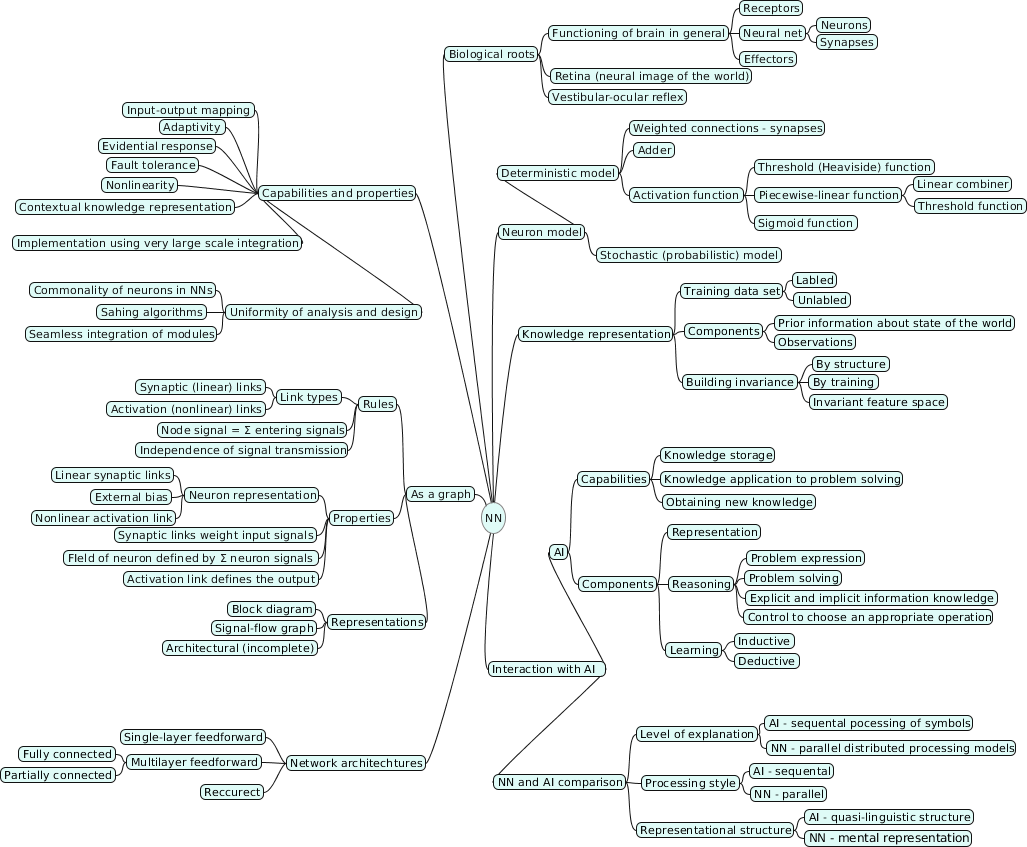
\includegraphics[width=1.0\textwidth]{NN}
\end{figure}

\section{Exercises}

\subsection{Exercise 1.1}

$\phi(v) = \frac{1}{1 + exp(-av)}$\\

Show that $\frac{d\phi(v)}{dv} = a\phi(v)[1 - \phi(v)]$. What is the value of this derivative at the origin?\\

Solution:\\

$\frac{d\phi(v)}{dv} = \frac{d((1 + exp(-av))^{-1})}{dv} = -\frac{-a\cdot exp(-av)}{(1 + exp(-av))^2} = \frac{a(exp(-av) + 1 -1)}{(1 + exp(-av))^2} = \frac{a}{(1 + exp(-av))} (1 - \frac{1}{(1 + exp(-av))}) = a\phi(v)[1 - \phi(v)]$\\

$\frac{a}{(1 + exp(-a\cdot 0))} (1 - \frac{1}{(1 + exp(-a\cdot 0))}) = \frac{a}{(1 + 1)} (1 - \frac{1}{(1 + 1)}) = \frac{1}{4}$


\subsection{Exercise 1.21}
Let x be an input vector and $s(\alpha, x)$ be a transformation operator acting on x and depending on some parameter $\alpha$. The operator $s(\alpha, x)$ satisfies:
\begin{itemize}
\item s(0, x) = x
\item $s(\alpha, x)$ is differential with respect to $\alpha$
\end{itemize}
How would you compute the tangent vector when $\alpha$ is small? The tangent vector is locally invariant with respect to rotation of the original image, why?\\

Solution:\\

Since $\alpha$ is small, we can use a Taylor expansion: $s(\alpha, x) = s(0, x) + \alpha \frac{\delta s(\alpha, x)}{\delta \alpha} + O(\alpha^2) \approx x + \alpha \frac{\delta s(\alpha, x)}{\delta \alpha}$\\

According, to the assignment, the tangent vector (V) is defined by the partial derivative $\frac{\delta s(\alpha, x)}{\delta \alpha}$, therefore:\\

$s(\alpha, x) =  x + \alpha V$\\

$V = \frac{s(\alpha, x) -  x}{\alpha}$\\

\end{document}
